
%(BEGIN_QUESTION)
% Copyright 2012, Tony R. Kuphaldt, released under the Creative Commons Attribution License (v 1.0)
% This means you may do almost anything with this work of mine, so long as you give me proper credit

An example of a SCADA component in an electric power system is the General Electric model PQM II power quality monitor.  This panel-mounted instrument inputs voltage and current signals from the power lines through instrument transformers (voltage and current step-down transformers), computing power factor, true power ($P$), reactive power ($Q$), apparent power ($S$), frequency, and imbalances of voltage or current between the different phases.  This device also has the ability to record and trend power system values over time.  A diagram showing the connections between a PQM II and the power lines is shown here:

$$\includegraphics[width=15.5cm]{i02030x01.eps}$$

Explain why {\it instrument transformers} (PTs and CTs with voltage step-down and current step-down ratios) are used to connect the PQM to the power system conductors.

\vskip 10pt

Assuming a phase-to-neutral voltage on ``B'' phase of 7155 volts AC, calculate the voltage seen between the PQM instrument's $V_2$ and $V_N$ terminals.

\vskip 10pt

Assuming a current of 148 amps AC through the ``C'' phase conductor of the power lines, calculate the current seen at the PQM instrument's Phase C ``5A'' terminal.

\vskip 10pt

Suppose you wished to connect a personal computer with a 9-pin serial port to the 9-pin serial port of the PQM.  Which terminals of each 9-pin serial port would you need to connect together, at minimum, to enable communication between the PQM and the PC?  Note: a personal computer is considered a DTE device, while the PQM is considered a DCE device!


\vskip 20pt \vbox{\hrule \hbox{\strut \vrule{} {\bf Suggestions for Socratic discussion} \vrule} \hrule}

\begin{itemize}
\item{} An important safety consideration when working with current transformers (CTs) is to {\it never} open-circuit the secondary winding of an energized CT.  Explain why.
\item{} An important safety consideration when working with current transformers (CTs) is to {\it never} short-circuit the secondary winding of an energized PT.  Explain why.
\item{} For those who have studied three-phase power circuits, calculate the line voltage of this system based on the 7155 VAC phase voltage presented above.
\item{} Are the PT primary windings connected together in a Wye or a Delta configuration?
\item{} Are the PT secondary windings connected together in a Wye or a Delta configuration?
\end{itemize}

\underbar{file i02030}
%(END_QUESTION)





%(BEGIN_ANSWER)

\noindent
{\bf Partial answers:}

\vskip 10pt

Explain why {\it instrument transformers} (PTs and CTs with voltage step-down and current step-down ratios) are used to connect the PQM to the power system conductors.  {\bf The instrument transformers provide both signal reduction and galvanic isolation between the PQM and the high-voltage, high-current power line conductors.}

\vskip 10pt

Assuming a phase-to-neutral voltage on ``B'' phase of 7155 volts AC, calculate the voltage seen between the PQM instrument's $V_2$ and $V_N$ terminals.  {\bf 119.25 volts}

%(END_ANSWER)





%(BEGIN_NOTES)

Explain why {\it instrument transformers} (PTs and CTs with voltage step-down and current step-down ratios) are used to connect the PQM to the power system conductors.  {\bf The instrument transformers provide both signal reduction and galvanic isolation between the PQM and the high-voltage, high-current power line conductors.}

\vskip 10pt

Assuming a phase-to-neutral voltage on ``B'' phase of 7155 volts AC, calculate the voltage seen between the PQM instrument's $V_2$ and $V_N$ terminals.  Each PT steps phase voltage down by a factor of 60:1, and so the ``B'' phase voltage of 7155 volts gets stepped down to {\bf 119.25 volts}.

\vskip 10pt

Assuming a current of 148 amps AC through the ``C'' phase conductor of the power lines, calculate the current seen at the PQM instrument's Phase C ``5A'' terminal.  Each CT steps line current dwn by a factor of 200:5 (40:1), and so the ``C'' line current of 148 amps gets stepped down to {\bf 3.7 amps}.

\vskip 10pt

Suppose you wished to connect a personal computer with a 9-pin serial port to the 9-pin serial port of the PQM.  Which terminals of each 9-pin serial port would you need to connect together, at minimum, to enable communication between the PQM and the PC?  Note: a personal computer is considered a DTE device, while the PQM is considered a DCE device! {\bf Connect pin 2 to pin 2, pin 3 to pin 3, and pin 5 to pin 5 (i.e. a ``straight'' cable rather than a ``null'' cable.}


\vfil \eject

\noindent
{\bf Summary Quiz:}

Suppose a technician measures 2.79 amps of current through the wire connected to the Multilin PQM unit's 
``Phase A (5A)'' terminal.  Calculate the amount of current going through the phase A power line conductor.

$$\includegraphics[width=15.5cm]{i02030x01.eps}$$

%INDEX% Measurement, power: GE Multilin PQM II power quality meter

%(END_NOTES)


